\documentclass{article}
\usepackage[utf8]{inputenc}
\usepackage[T1]{fontenc}
\usepackage[portuguese]{babel}

\usepackage{indentfirst}
\usepackage{makeidx}
\usepackage{stackengine}
\usepackage{amssymb}
\usepackage{amsthm}
\usepackage{hyperref}
\usepackage{color}
\usepackage{graphicx}

\usepackage{pdfpages}

\usepackage{booktabs}

\title{\bf{Aprendizagem Computacional - Trabalho Prático 3}\vspace{80mm}}
\author{\textbf{João Tiago Márcia do Nascimento Fernandes - 2011162899} \\
\textbf{Joaquim Pedro Bento Gonçalves Pratas Leitão - 2011150072}}
\makeindex

\begin{document}

\maketitle

\pagebreak

\renewcommand*\contentsname{Índice}
\tableofcontents

\pagebreak

\section{Introdução}

O presente trabalho foca-se na previsão e identificação de crises epiléticas, com base em informação de sinais cerebrais, recolhidos através da realização de um \emph{EEG} (ElectroEncefaloGrama).

Este exame recolhe dados relativos à atividade cerebral do paciente que o realiza, sendo possível extrair um conjunto de características que permite a identificação de momentos de ocorrência de crises epiléticas (denominadas situações \emph{ictais}) e de momentos nos quais o paciente não apresenta qualquer problema (denominadas situações \emph{não-ictais}).

O trabalho proposto visa a criação de uma aplicação em \emph{Matlab}, que analise os dados recolhidos após a realização de um \emph{EEG} a um paciente, e que identifique eventuais situações em que a atividade cerebral registada corresponde a uma situação de crise epilética.

Para proceder à identificação das situações \emph{ictais} e \emph{não-ictais}, a aplicação desenvolvida faz uso, na sua arquitetura interna, de redes neuronais, disponíveis na \emph{Neural Networks Toolbox} do próprio \emph{Matlab}.

Para avaliar o desempenho e performance da aplicação desenvolvida, procederemos à análise da sensibilidade e especificidade de cada rede neuronal implementada.

Estas métricas correspondem à percentagem de situações \emph{ictais} verdadeiras detetadas (\emph{sensibilidade}) e à percentagem de situações \emph{não-ictais} falsas detetadas (\emph{especificidade}), refletindo a performance da rede na classificação de um dado \emph{data set}: Uma elevada \emph{sensibilidade} implica uma boa deteção de situações \emph{ictais}, enquanto que uma elevada \emph{especificidade} implica uma boa deteção de casos \emph{não-ictais}.

Ambas as métricas constituem requisitos necessários para a sua utilização em ambiente clínico, e podem ser definidas da seguinte forma:

$$Sensibilidade \: = \frac{PositivosVerdadeiros}{PositivosVerdadeiros + FalsosNegativos}$$

$$Especificidade \: = \frac{NegativosVerdadeiros}{NegativosVerdadeiros + FalsosPositivos}$$

\vspace{.1cm}

No presente documento pretendemos apresentar de forma mais detalhada a aplicação desenvolvida, discutindo alguns detalhes da sua implementação e apresentando uma reflexão crítica sobre o seu desempenho e performance, nomeadamente da sua sensibilidade e especificidade.

\pagebreak

\section{Aplicação Desenvolvida}

Tal como referido anteriormente, a aplicação desenvolvida visa analisar os dados referentes a um \emph{EEG} de um paciente, identificando situações correspondentes a uma crise epilética.

Esta classificação pode ser realizada de duas formas distintas, que passamos a descrever.

Numa primeira abordagem, a que chamamos \emph{Classificação Individual}, é atribuído a cada elemento do conjunto de dados de entrada da aplicação uma de duas \emph{classes}, representadas por dois valores binários:

\begin{itemize}
\item Classe \emph{não-ictal}, correspondente a um estado normal do paciente (ausência de crises) e representada pelos valores \emph{1 0}

\item Classe \emph{ictal}, correspondente a uma situação de crise, e representada pelos valores \emph{0 1}
\end{itemize}

Na segunda abordagem, a que chamamos \emph{Classificação em Grupo}, o processo de classificação das entradas é realizado de forma semelhante, no entanto são considerados conjuntos de dados de entrada da aplicação, ao invés de cada elemento. Para este tipo de classificação podemos adotar duas métricas diferentes:

\begin{itemize}
\item Analisar o número de elementos consecutivos classificados individualmente como \emph{ictais}, comparando-o com um dado limiar. Neste caso, se, por exemplo, existirem pelo menos 10 elementos consecutivos classificados como \emph{ictais} então é detetada uma crise. Caso contrário nenhuma crise é detetada.

\item Adotar um sistema de classificação em janela deslizante, analisando o número de elementos classificados individualmente como \emph{ictias}, num dado universo restrito. Isto é, se pelo menos cinco dos últimos dez elementos foram classificados como \emph{ictais} então todos os elementos nesse conjunto são classificados como \emph{ictais}.
\end{itemize}

Optámos por adotar o segundo método de \emph{Classificação em Grupo}, considerando uma abordagem por janelas, uma vez que o primeiro método, na nossa opinião, não torna o classificador resistente a variações no tempo. Isto é, caso a saída obtida seja igual à esperada, mas com todos os elementos deslocados, por exemplo, em uma unidade este método irá considerar um número de classificações erradas muito maior do que numa abordagem por janelas.

De seguida apresentamos em maior detalhe a aplicação desenvolvida, salientando alguns dos seus aspetos mais importantes e relevantes.

\subsection{Graphical User Interface}

Para facilitar a interação do utilizador com a aplicação, foi-nos proposta a criação de uma interface gráfica onde são solicitadas ao utilizador todas as informações relevantes para a execução da aplicação, separando por completo a sua lógica interna com a especificação dos seus dados de entrada e outros parâmetros.

Assim, na interface gráfica desenvolvida são solicitadas ao utilizador várias informações que permitem a criação e treino das diferentes redes neuronais, nomeadamente:

\begin{itemize}
\item Tipo de rede neuronal a criar e treinar. Encontram-se disponíveis as redes \emph{Radial Basis Function}, \emph{Layer Recurrent Network}, \emph{FeedForward}, \emph{FeedForward Time Input Delay} e \emph{Distributed Time Delay}.

\item Função de Aprendizagem (ou Função de Treino) a utilizar na rede neuronal a criar (Se necessário). Encontram-se disponíveis as funções \emph{trainscg}, \emph{traingd} e \emph{trainrp}.

\item Função de Performance a utilizar no treino da rede neuronal (se necessário). Estão disponíveis as funções \emph{mse} (mean squared error) e \emph{sse} (sum squared error).

\item Função de Activação dos neurónios da rede neuronal a implementar (se necessário). Estão disponíveis as funções \emph{hardlim}, \emph{purelin}, \emph{logsig} e \emph{tansig}.

\item Tipo de Classificação a realizar (\emph{Individual} ou \emph{Em Grupo})

\item Ficheiro de dados a utilizar para treinar a rede criada

\item Ficheiro de dados a utilizar para testar a rede criada

\item Número de características dos pacientes a considerar

\item Outros aspetos, como objetivo do treino (\emph{Goal}), taxa de aprendizagem, etc
\end{itemize}

Para além disso, na interface desenvolvida, existe também uma secção onde são apresentados os resultados de cada teste realizado, nomeadamente a especificidade e sensibilidade da rede considera.

\begin{figure}[h]
  \centering
      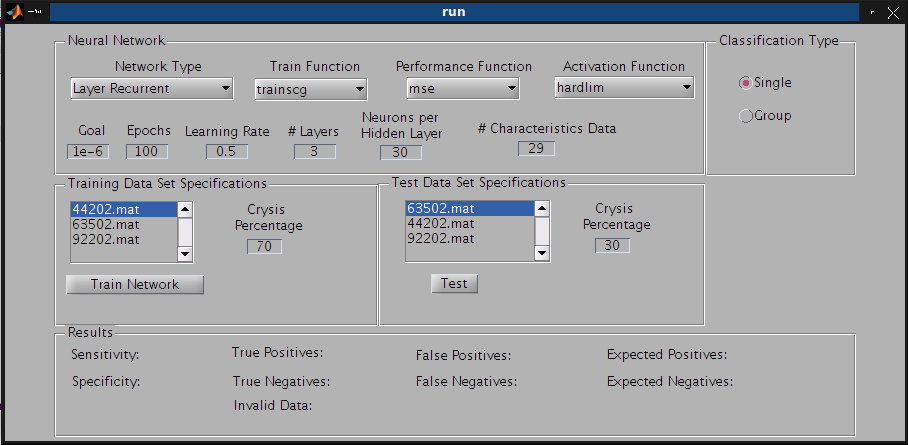
\includegraphics[scale=0.3]{Images/Aplication_GUI.png}
  \caption{Interface Gráfica implementada}
\end{figure}

\subsection{Redes Neuronais Implementadas}

Como já referimos anteriormente, na nossa aplicação implementámos cinco redes neuronais distintas: \emph{Radial Basis Function}, \emph{Layer Recurrent Network}, \emph{FeedForward}, \emph{FeedForward Time Input Delay} e \emph{Distributed Time Delay}.

Estas redes apresentam, naturalmente, características e propriedades distintas, sendo que umas se adequam mais ao trabalho que pretendemos realizar do que outras.

Por exemplo, considerando a rede \emph{Layer Recurrent}, esta rede permite a introdução de atrasos em algumas características, o que lhe permite aprender a prever qualquer saída dinâmica, tendo por base entradas passadas. Este processo é possível se forem considerados neurónios e atrasos suficientes na rede.

De facto, esta é uma propriedade que vai, de certa forma, ao encontro do funcionamento de um cérebro humano, que para além de ser um sistema dinâmico, possui também memória.

Na mesma linha de raciocínio, redes que suportam a introdução de atrasos em algumas das características que constituem os dados de entrada surgem, a uma primeira vista, como boas opções para simular o comportamento de um cérebro humano, realizando uma melhor identificação das situações correspondentes a crises epiléticas. Exemplos destas redes são a rede \emph{Distributed Time Delay} e a \emph{FeedForward Input Time Delay}.

Por seu turno, a rede \emph{FeedForward} também se apresenta como uma solução a considerar, dado o facto de permitir uma boa implementação de qualquer função de entradas e saídas arbitrárias, desde que considerados neurónios suficientes na(s) camada(s) escondida(s).

Por fim, é também necessário referir a rede \emph{Radial Basis Function}, bastante utilizada para aproximar funções e cujo treino passa nomeadamente pela adição de neurónios à camada escondida até que a rede atinja a performance (\emph{goal}) pretendida. Assim, embora possa ser necessário adicionar um elevado número de neurónios à camada escondida, acreditamos ser possível ter uma boa performance com esta rede.

\subsection{Treino das Redes}

Um dos principais aspetos do trabalho realizado, prende-se com o treino das redes neuronais, pois é ele que determina a boa (ou má) performance das redes implementadas.

Para o presente trabalho foram-nos fornecidos dados relativos a três pacientes, constituídos por um conjunto de características extraídas para cada elemento, e pela respetiva classe definida para cada elemento.

Uma vez que as situações em que os pacientes estão a sofrer de uma crise epilética são consideravelmente menos do que as situações em que o paciente não apresenta nenhum problema, a simples seleção de todos os elementos de um dos conjuntos fornecidos, ou de parte desses elementos, para realizar o treino da rede, sem qualquer cuidado na seleção dos elementos irá conduzir a dados de treino onde predominam situações \emph{não-ictais}.

Nesses casos, iremos verificar uma especialização da rede na identificação de situações \emph{não-ictais}, sem que faça uma classificação de casos \emph{ictais} igualmente fiável.

De facto, tal situação não é desejável, uma vez que o nosso principal objetivo passa pela identificação de casos \emph{ictais} com um grau de confiança mínimo, não a identificação de situações \emph{não-ictais}.

Assim, para evitar que as redes por nós treinadas se especializem em situações \emph{não-ictais}, na constituição dos casos de treino das diferentes redes neuronais, consideramos um dos ficheiros fornecidos, e para esse ficheiro selecionamos uma percentagem dos casos \emph{ictais} (essa percentagem é solicitada ao utilizador através da interface gráfica) que vamos incluir no nosso \emph{data set} de treino.

Em seguida, selecionamos um número igual de situações \emph{não-ictais}, preservando a ordem dos diferentes casos nos dados originais. Como o número de situações \emph{não-ictais} é bastante superior ao número de situações \emph{ictais}, ao selecionarmos um número de situações \emph{não-ictais} igual ao de situações \emph{ictais} temos, necessariamente de não incluir a maior parte das situações \emph{não-ictais}.

Para além disso, consideremos duas características observadas em dois momentos distintos do exame: Uma, observada num momento em que o paciente se encontra clinicamente estável (portanto numa situação \emph{não-ictal}); E outra, observada instantes antes da ocorrência de uma crise.

Embora ambas as situações sejam classificadas como \emph{não-ictais}, facilmente compreendemos que a segunda se encontra mais próxima de um estado \emph{ictal}, do que a primeira. Efetivamente, para evitar que as redes por nós treinadas classifiquem estas duas situações apresentadas com diferentes valores (atribuindo à primeira a classificação de \emph{não-ictal} e à segunda de \emph{ictal}), é necessário incluir, nos dados de treino das redes, uma porção de características que reflitam ambas as situações apresentadas, a par das situações \emph{ictais}.

Assim, para fazermos a seleção dos dados de treino das nossas redes, selecionamos aleatoriamente um conjunto de situações \emph{não-ictais} do conjunto de dados originais, preservando sempre a ordem de ambas as situações \emph{ictais} e \emph{não-ictais}, e assegurando a inclusão de exemplos referentes às duas situações apresentadas.

No processo de treino das redes recorremos ainda a diferentes funções de treino, disponíveis e implementadas pela \emph{Neural Network Toolbox} do \emph{Matlab}. As funções de treino disponíveis são a função \emph{traingd}, \emph{trainscg} e \emph{trainrp}.

Com exceção da rede \emph{RBF} (\emph{Radial Basis Function}) implementada, o treino das restantes redes neuronais é realizado com recurso à função \emph{train} da \emph{Neural Network Toolbox} do \emph{Matlab}. Uma vez que o treino das redes é uma operação complexa e exigente em termos computacionais, tendo em conta o tipo de redes criadas e a dimensão dos dados para proceder ao treino das redes, estas foram treinadas com aceleração gráfica, disponível nas versões mais recentes do \emph{Matlab}. Para tal, basta adicionar os parâmetros \emph{'useGPU', 'yes'} aquando da chamada da função \emph{train}: \emph{train(network, P, T, 'useGPU', 'yes')}.

Para a rede \emph{RBF}, o \emph{Matlab} realiza o seu treino aquando da criação da rede, não sendo necessária a invocação da função \emph{train}.

\subsection{Teste das Redes}

Uma vez completo o treino de uma rede neuronal, esta pode ser testada, de forma a verificar o seu bom, ou mau, funcionamento. Para isso, criámos um conjunto de dados de teste, baseados nos três \emph{data sets} inicialmente fornecidos.

O processo de criação dos dados de teste é semelhante ao utilizado na constituição dos dados de treino das redes neuronais:

É solicitado ao utilizador que indique o ficheiro (de entre os três ficheiros fornecidos) de onde serão extraídos os dados de teste, e qual a percentagem de situações \emph{ictais} a incluir. Em seguida, o ficheiro escolhido é analisado, e são considerados todos os dados nele presentes, a partir do final do ficheiro, até que o número de situações \emph{ictais} incluídas seja igual à percentagem especificada.

Por outras palavras, se o utilizador especifica que pretende incluir $25\%$ das situações \emph{ictais} nos dados de treino, e se todas as situações \emph{ictais} identificadas nesse \emph{data set} se encontram nas posições $10-20$, $40-50$, $60-70$ e $80-100$, então o nosso \emph{data set} de treino será constituído por todos os elementos do ficheiro, desde a posição $60$ até ao final do ficheiro.

Uma vez que aquando da realização dos testes na rede esta já se encontra treinada, é irrelevante considerarmos nos \emph{data sets} de teste situações \emph{ictais} na mesma ordem de grandeza do que situações \emph{não-ictais}, pois apenas estamos a executar a rede para um conjunto de dados, sem que este afete de forma alguma o funcionamento da rede em situações futuras.

\subsection{Implementação em Matlab}

A aplicação foi por nós desenvolvida e programa quase na sua totalidade, com a exceção do código relativo à interface gráfica. Esta foi desenhada por nós através da interface \emph{guide} do \emph{Matlab}, tendo o seu código sido gerado pelo \emph{Matlab}.

De qualquer forma, toda a lógica interna da aplicação, comunicação da informação recolhida pela interface gráfica para outras estruturas, etc, foi por nós completamente desenvolvida.

\subsubsection{run.m}

Este é o principal ficheiro da aplicação e que permite a sua execução. É nele que se encontra todo o código gerado, relativo à interface gráfica, mas também onde todas as principais funcionalidades da aplicação (criação das redes neuronais e respetivo treino e classificação dos dados de teste) são invocadas.

\subsubsection{createNetwork.m}

No ficheiro \emph{createNetwork.m} encontramos a função \emph{createNetwork}, responsável pela criação da rede neuronal que irá realizar a identificação das  situações \emph{ictais} nos dados considerados e fornecidos à aplicação. 

Esta rede é criada de acordo com algumas características pré-definidas, e outras escolhidas pelo utilizador, como é o caso das funções de ativação e de treino.

Após a sua criação, a rede será treinada com um conjunto de dados previamente criado de acordo com as especificações fornecidas pelo utilizador. Este treino não é realizado neste ficheiro, mas sim no principal ficheiro desenvolvido para a aplicação, \emph{run.m}.

\subsubsection{prepareDataSets.m}

Neste ficheiro encontramos a função \emph{prepareDataSets}, responsável pela criação dos \emph{data sets} de treino e e de teste, bem como dos respetivos resultados esperados (quer para os dados de treino, quer para os dados de teste). Para além disso, neste ficheiro é ainda invocado o procedimento responsável pela seleção das principais características registadas, para o paciente em questão, que abordaremos em maior detalhe mais à frente nesta secção.

Tal como referimos brevemente numa secção anterior do presente documento, as abordagens seguidas para a criação dos conjuntos de dados de treino e de teste têm pontos em comum, não sendo, no entanto, completamente iguais.

Uma vez que, nos ficheiros fornecidos, o número de situações \emph{não-ictais} é bastante superior à quantidade de classificações \emph{ictais}, se simplesmente considerarmos para o nosso \emph{data set} de treino uma percentagem dos dados fornecidos, sem nos preocuparmos com a distribuição de situações \emph{não-ictais} e \emph{ictais}, então será altamente provável que as nossas redes sejam treinadas com mais casos \emph{não-ictais} do que com \emph{ictais}, resultando numa especialização da mesma na deteção de situações \emph{não-ictais}.

Efetivamente, tal situação corresponde ao oposto do desejável, tendo em conta que o nosso objetivo principal passa pela identificação de casos \emph{ictais}, com um grau de confiança mínimo.

Assim, para os dados de treino das redes neuronais criadas são consideradas situações \emph{ictais} e \emph{não-ictias} em igual número e de acordo com uma percentagem das situações \emph{ictais} totais do ficheiro a considerar, definida pelo utilizador. Nesta seleção, tal como referido anteriormente, é preservada a posição relativa das situações \emph{ictais} e \emph{não-ictais} consideradas, e assegurando a inclusão de exemplos referentes Às duas situações \emph{não-ictais} apresentadas.

No que respeita aos dados de teste, também criados neste ficheiro, não é necessária qualquer preocupação em relação ao número de situações \emph{ictais} e \emph{não-ictais}, uma vez que pretendemos utilizar estes dados em redes já treinadas, pelo que a sua execução em nada alterará o comportamento futuro da rede.

Assim, os dados de treino são construídos partindo do final de um ficheiro de dados previamente selecionado, incluindo todos os dados (correspondentes a casos \emph{ictais} e \emph{não-ictais}) até que o número de situações \emph{ictais} seja igual a um valor definido pelo utilizador.

\subsubsection{processCharacteristics.m}

Neste ficheiro podemos encontrar o procedimento responsável pela seleção das principais características registadas, para o paciente em questão.

Esta seleção é feita com base numa análise da correlação entre as diferentes características registadas e a classificação esperada para cada conjunto, selecionando as características que apresentam valores de correlação mais elevados, e em número igual ao especificado pelo utilizador na interface gráfica.

Com este procedimento pretendemos eliminar características redundantes dos nossos ficheiros de dados. Embora seja de prever que esta eliminação em nada altere a aprendizagem da rede (ou, em caso de alteração, que esta seja bastante ténue), é expectável uma melhoria no seu tempo de treino proporcional ao número de características redundantes removidas.

\subsubsection{interpretResults.m}

É neste ficheiro que se encontra a função \emph{interpretResults}, onde é realizado o processamento da classificação executada pela rede neuronal treinada, nas situações em que o tipo de classificação escolhido é a \emph{Classificação Individual}.

Este processamento consiste simplesmente em percorrer os resultados obtidos na execução da rede neuronal para o caso de teste fornecido, comparando-os elemento a elemento com os resultados esperados para esse caso de teste. Assim, é registado o número de situações em que a classificação da rede se apresenta correta (distinguindo-se entre classificações de situações \emph{ictais} e \emph{não-ictais}), bem como situações em que a classificação da rede está incorreta (também distinguindo-se entre ituações \emph{ictais} e \emph{não-ictais}).

Para além disso, são também registados o número de classificações positivas e negativas, isto é, de situações \emph{ictais} e \emph{não-ictais}, presentes nos dados fornecidos à rede, e que num cenário de classificação perfeita corresponderiam ao número de situações \emph{ictais} e \emph{não-ictais} registadas.

Uma vez que a classificação realizada pela rede nem sempre é clara, podem existir situações para as quais a rede não convergiu, não sendo possível distinguir de forma clara para uma dada situação (ou conjunto de situações) qual a classe atribuída pela rede. Essas situações são também registadas nesta função, sendo posteriormente reportadas como classificações inválidas.

\subsubsection{interpretGroupResults.m}

O ficheiro \emph{interpretGroupResults.m} é responsável por uma importante parte da lógica subjacente à \emph{Classificação em Grupo} realizada pela aplicação.

Neste ficheiro, a abordagem seguida é em tudo semelhante ao realizado no caso da \emph{Classificação Individual}: Possuindo os resultados esperados para o teste realizado, basta percorrer os dados obtidos como resultado da classificação da rede neuronal, registando as situações em que os dois conjuntos de dados (dados obtidos e esperados) são idênticos (verdadeiros positivos e verdadeiros negativos), bem como situações onde as classificações diferem (falsos positivos e falsos negativos), ou então não são possíveis (classificações inválidas).

\subsection{Execução}

Para executar a aplicação o utilizador simplesmente necessita de executar o ficheiro \emph{run.m}, sendo imediatamente exibida a interface gráfica desenvolvida.

A partir desse momento, o utilizador poderá escolher a rede a criar e a treinar, definindo algumas das suas propriedades e do seu treino, nomeadamente a escolha do ficheiro de dados a utilizar como fonte para a criação dos dados de treino e para posterior teste da rede treinada. É também possível selecionar o tipo de classificação a realizar, e o número de características a considerar.

Uma vez definidos todos os parâmetros pretendidos pelo utilizador, basta clicar na opção \emph{Train Network}, para proceder ao treino da rede, ou na opção \emph{Test}, para proceder à execução da rede para os dados de teste especificados.

Queremos também salientar a possibilidade de seleção a opção \emph{Test} sem, previamente, ter sido treinada nenhuma rede. Nesse caso, será criada e treinada uma rede de acordo com as especificações para esta definidas na interface. Caso o utilizador não tenha definido nenhuma configuração, será utilizada uma por defeito.

Uma vez finda a execução da rede para os dados de treino selecionados, os resultados dessa execução poderão ser visualizados no painel \emph{Results}, estando disponível a \emph{sensibilidade} e \emph{especificidade} registadas, bem como os dados que permitiram calcular esses valores (verdadeiros positivos e negativos, e falsos positivos e negativos). É ainda apresentado o número de classificações inválidas registadas. 

\pagebreak

\section{Treino e Testes da Aplicação}
\label{sec:train_tests}

Após o desenvolvimento inicial da aplicação procedemos ao treino e teste das diferentes redes implementadas, a fim de aferir o seu correto, ou incorreto, funcionamento e da sua adequação às nossas previsões iniciais para a performance de cada rede.

\subsection{Testes Iniciais}

\subsubsection{Descrição}

\textbf{Reformular a partir daqui}

Numa fase inicial dos testes realizados procedemos ao treino de todas as redes neuronais implementadas, para uma vasta gama de combinações possíveis das propriedades das redes consideradas, e para os dois tipos de classificação disponíveis. Assim, inicialmente treinámos as redes com as seguintes propriedades: 

\begin{itemize}
\item Dados de treino retirados do ficheiro \emph{92202.mat}

\item Percentagem de situações \emph{ictais} consideradas nos casos de treino de $70\%$

\item Objetivo do treino com o valor de $10^{-6}$, com exceção da rede \emph{Radial Basis Function}, onde o valor considerado foi de $10^{-2}$

\item Número de épocas de treino máximo de $1000$

\item Número de \emph{validation checks} necessários para terminar o treino igual a metade do número máximo de épocas de treino, ou seja $500$

\item Ritmo de aprendizagem de $0.2$

\item Número de Camadas Totais igual a $4$ (incluindo a camada de saída)

\item Número de neurónios por cada camada escondida (excluindo a camada de saída) igual a $30$

\item Funções de ativação consideradas: \emph{hardlim}, \emph{purelin}, \emph{logsig} e \emph{tansig}

\item Funções de treino consideradas: \emph{trainscg}, \emph{traingd} e \emph{trainrp}

\item Funções de performance consideradas: \emph{sse} e \emph{mse}
\end{itemize}

Antes de entrarmos em maior detalhe sobre os testes realizados gostaríamos de referir alguns pontos que consideramos importantes para uma posterior análise.

Em primeiro lugar, gostaríamos de chamar a atenção do leitor para o número de camadas consideradas nos testes realizados: Um dos pontos defendidos pela bibliografia deste tema refere-se ao facto de, numa rede neuronal com uma única camada escondida (excluindo a camada de entrada e a de saída), ser possível obter os mesmos resultados que numa rede neuronal equivalente, mas que faça uso de mais camadas.

Simplesmente para obter resultados equivalentes é necessário adicionar um número suficiente de neurónios à camada escondida. Naturalmente que, ao se adicionar um elevado número de camadas e de neurónios por camada, o tempo de treino da rede aumenta consideravelmente.

Para além disso, analisando o número de camadas e de neurónios por camada considerados, este pode parecer demasiado excessivo. Efetivamente, numa fase posterior da nossa análise, iremos considerar algumas destas redes treinadas com um número de camadas e de neurónios por camada bastante mais reduzido, com intenção de compararmos os resultados obtidos em cada situação.

Com o objetivo de aferir a validade das redes implementadas, iniciamos os testes executando as diferentes redes para os dados do ficheiro \emph{92202.mat} não utilizados para o treino da rede. Dado que estes dados são relativos ao mesmo paciente com o qual as redes foram treinadas será de prever que estes dados se aproximem mais dos dados de treino das redes, resultando numa melhor performance.

Posteriormente a este teste, foram também executados testes com os dados relativos a outros dois pacientes, considerando para efeitos de teste porções de $30\%$, $50\%$ e $70\%$ do número total de situações \emph{ictais} presentes em cada um dos ficheiros.

Em anexo a este documento encontra-se uma lista detalhada dos resultados obtidos em cada teste realizado, que poderá ser consultada pelo leitor.

Na lista apresentada optámos por não incluir os resultados relativos aos testes para as redes treinadas com a função \emph{sum squared error} como função de performance, uma vez que as redes treinadas com esta função obtiveram valores de performance registados pela \emph{Neural Network Toolbox} muito superiores aos registados para as redes treinadas com a função de performance \emph{mean squared error}\footnote{Neste caso, quanto maior for o valor registado para a performance de uma rede pior será o seu desempenho}

\subsubsection{Análise dos Resultados Obtidos}

Analisando os resultados obtidos neste teste, existem alguns pontos que, na nossa opinião, se tornam evidentes e que gostaríamos de salientar, desde já.

Nos testes realizados com os dados provenientes do ficheiro \emph{92202.mat} não utilizados no treino das redes, ficámos algo surpreendidos com os resultados obtidos.

De uma forma geral, todas as redes apresentam, nesta situação, valores de \emph{especificidade} bastante elevados (excluindo algumas situações pontuais). No entanto, os valores de \emph{sensibilidade} registados são bastante reduzidos e irregulares. Queremos também chamar a atenção para o facto de, nos testes realizados, a rede \emph{Radial Basis Function} não ter realizado uma única classificação inválida, o que é algo que consideramos bastante positivo.

De facto, tal como referimos, seria de esperar que as redes realizassem boas classificações para casos próximos dos com que foram treinadas, como é o caso quando consideramos dados do mesmo paciente. Embora essa situação se verifique, em algumas situações, para os valores de \emph{especificidade}, os valores de \emph{sensibilidade} e também o número de classificações inválidas revelam outra realidade.

Tais resultados sugerem, assim, a possível existência de um erro na implementação destas redes ou, numa situação mais improvável, a possibilidade de, acidentalmente, termos corrompido os dados no ficheiro que utilizámos para o treino da rede, antes ou depois desse mesmo treino.

No entanto, e tal como iremos constatar de seguida, os resultados obtidos quando sujeitamos as redes a outros dados de teste não foram tão negativos.

Numa primeira e superficial análise, seria plausível considerar que, à luz dos resultados obtidos para os restantes pacientes analisados, a maioria das redes implementadas apresenta uma boa capacidade de generalização. No entanto, os resultados que acabámos de apresentar não nos deixam tão confiantes.

Não obstante, passemos à análise da prestação das diferentes redes, quando executadas com dados diferentes dos com que foram treinadas.

Em primeiro lugar, queremos desde já destacar o facto de, também neste conjunto de testes, não ter sido registada nenhuma classificação inválida por parte da rede \emph{Radial Basis Function}.

Para além disso, verificámos que os resultados obtidos para a \emph{Classificação Individual} e \emph{Classificação em Grupo} são bastante semelhantes. De facto, este é, de certa forma, um resultado pouco surpreendente, dado que a nossa abordagem para a \emph{Classificação em Grupo} é bastante semelhante à abordagem para a \emph{Classificação Individual}. Todos os passos desde a criação dos dados de teste até à sua execução na rede são comuns aos dois tipos de classificação. A única diferença reside na forma como estes são processados após a sua execução na rede neuronal.

Como os nossos dados possuem as situações \emph{ictais} bastante concentradas em locais muito específicos dos \emph{data sets}, e uma vez que optámos pela abordagem em janela para a \emph{Classificação em Grupo}, esta semelhança entre os resultados obtidos nas duas abordagens não completamente inesperada.

Não obstante, gostaríamos também de salientar que, embora os resultados obtidos para os dois tipos de classificações sejam bastante semelhantes, registámos melhores resultados nos testes que relativos à \emph{Classificação Individual}.

De entre todas as redes testadas, aquela que apresentou melhores e mais consistentes resultados em ambos os tipos de classificação foi, sem dúvida, a rede \emph{Radial Basis Function}, apresentando em praticamente todos os testes elevados valores (iguais ou superiores a $0.7$) de especificidade e sensibilidade.

Para além desta rede, na \emph{Classificação Individual} registámos ainda bons resultados para a rede \emph{Distributed Time Delay}, treinada com a função \emph{trainscg}, tal como a rede \emph{FeedForward Input Time Delay}, em algumas situações pontuais (nomeadamente utilizando como função de treino a função \emph{trainscg} e funções de ativação as funções \emph{logsig} e \emph{tansig}).

As restantes redes e respetivas configurações não mencionadas, não obtiveram resultados tão positivos, destacando-se sobretudo uma clara irregularidade nos resultados registados: Foi bastante frequente a ocorrência de situações em que uma dada rede registava um valor bastante elevado para a especificidade ou para a sensibilidade, mas o correspondente valor de sensibilidade ou de especificidade registado tomava valores muito reduzidos.

Surpreendentemente, nas redes que apresentam piores resultados, onde se incluem as redes que apresentam as oscilações de resultados que referimos, é bastante comum registarem-se percentagens de dados inválidos mais reduzidas do que em algumas redes com melhores resultados.

No que diz respeito à \emph{Classificação em Grupo}, os resultados obtidos não são demasiado diferentes dos mencionados. Queremos destacar, à semelhança do que verificámos para a \emph{Classificação Individual}, a boa performance da rede \emph{Radial Basis Function}, e da rede \emph{Layer Recurrent Network}, que desta feita relegou a rede \emph{Distributed Time Delay}, treinada com a função \emph{trainscg} para o posto de terceira melhor rede.

À semelhança do verificado na \emph{Classificação Individual}, a rede \emph{FeedForward Input Time Delay} registou bons resultados em alguns testes onde foi treinada com a função \emph{trainscg}, tendo sido utilizadas as funções de ativação \emph{logsig} e \emph{tansig}.

Também se verificou uma grande oscilação nos resultados obtidos para algumas redes, registando-se situações em que, uma dada rede, foi registado um valor bastante elevado para a especificidade ou para a sensibilidade, mas o correspondente valor de sensibilidade ou de especificidade era muito mais reduzido.

Quanto ao número de classificações inválidas, registámos valores, em média, inferiores aos da \emph{Classificação Individual}, existindo muitas redes que não apresentam qualquer classificação inválida.

Curiosamente, são as redes com maiores oscilações de valores de sensibilidade e especificidade que apresentam os maiores valores de classificações inválidas.

\subsection{Testes Complementares}

Tendo em conta os testes realizados para dados diferentes dos dados de treino, decidimos avaliar um pouco mais as redes que mostraram um melhor desempenho, realizando pequenas alterações às suas configurações, repetindo os treinos realizados e analisando os resultados.

\subsubsection{Redes Selecionadas}

Assim, nesta segunda fase de testes, consideramos as seguintes redes neuronais:

\begin{itemize}
\item Rede \emph{Radial Basis Function}, com um \emph{goal} de $0.01$, um neurónio a adicionar entre \emph{displays}

\item Rede \emph{Distributed Time Delay}, treinada com a função \emph{trainscg}, e com as funções de ativação \emph{logsig} e \emph{tansig}

\item Rede \emph{FeedForward Input Time Delay}, treinada com a função \emph{trainscg}, e com as funções de ativação \emph{logsig} e \emph{tansig}
\end{itemize}

Todas estas redes foram treinadas com apenas uma camada escondida e com $3$, $7$ e $15$ neurónios por camada. Para além disso, com exceção da rede \emph{Radial Basis Function}, foi utilizado um \emph{goal} de $10^{-6}$, $1000$ \emph{epochs} e um limite máximo de \emph{validation checks} de $500$ para o treino das redes.

Para os testes realizados, as redes foram executadas considerando os ficheiros \emph{44202.mat} e \emph{63502.mat}, selecionando $30$, $50$ e $70\%$ das situações \emph{ictais} registadas em cada um desses ficheiros.

De uma forma geral, os resultados da \emph{Classificação Individual e em Grupo} não sofreram muitas alterações, face ao verificado para as respetivas redes nos testes anteriormente realizados:

A rede \emph{Radial Basis Function} continuou a não registar dados inválidos, mesmo quando o seu número de neurónios foi reduzido a $3$, o que, na nossa opinião, é um ponto positivo.

Verificaram-se também algumas variações nos valores de \emph{sensibilidade} e \emph{especificidade} registados, no entanto não existiu nenhum teste em particular onde os valores registados para estas métricas se afastassem por completo do observado nos testes anteriores.

Tendo em conta estes resultados, podemos constatar que as redes escolhidas para este segundo conjunto de testes realizam classificações com o mínimo de confiança, uma vez que mesmo quando constituídas por um reduzido número de neurónios, mantiveram valores de \emph{sensibilidade} e \emph{especificidade} elevados.

Isto leva-nos a acreditar que a sua estrutura, bem como as funções de treino e ativação consideradas conferem a estas redes uma boa capacidade para identificar situações \emph{ictais} na atividade cerebral humana, adequando-se e permitindo simulando com alguma proximidade a atividade do cérebro humano, pelo menos no que respeita aos seus estados \emph{ictais} e \emph{não-ictais}.

\subsection{Redução da Dimensionalidade}

Explicar a ideia por trás disto (Muitas características com informação redundante --> Filtrando as que dão mais ganhos informativos ao sistema podemos ter uma aprendizagem ligeiramente pior, ou até igualmente melhor, necessitando de menos tempo para o treino da rede)

\textbf{FIXME: MUDAR INTERFACE GRAFICA PARA PERMITIR UTILIZAR REDIMENSIONALIZAÇÃO DOS DADOS}

%Testes segunda abordagem --> Reduzir dimensionalidade. Para esses testes já temos scripts para treinar as redes e para executar os testes, é só mesmo actualizar os datasets de treino e de teste... Depois meter a parte da redução da dimensionalidade num script, e outro para treinar as redes, etc. Para já não incluímos isso na aplicação, apresentamos isso como uma coisa independente da aplicação mas se tivermos tempo podemos fazer isso na interface, e depoisé adicionar campos no relatório onde explicamos isso

\pagebreak

\section{Conclusões}

Falar na generalização, uma vez que tivemos bons resultados (lol) em dados de pacientes que não o paciente de treino.

Referir os resultados menos positivos obtidos nos testes com os dados do paciente de treino.


\pagebreak

\section{Anexos}

Nas páginas seguintes apresentamos os testes iniciais realizados para \emph{Classificação Individual e em Grupo}, 

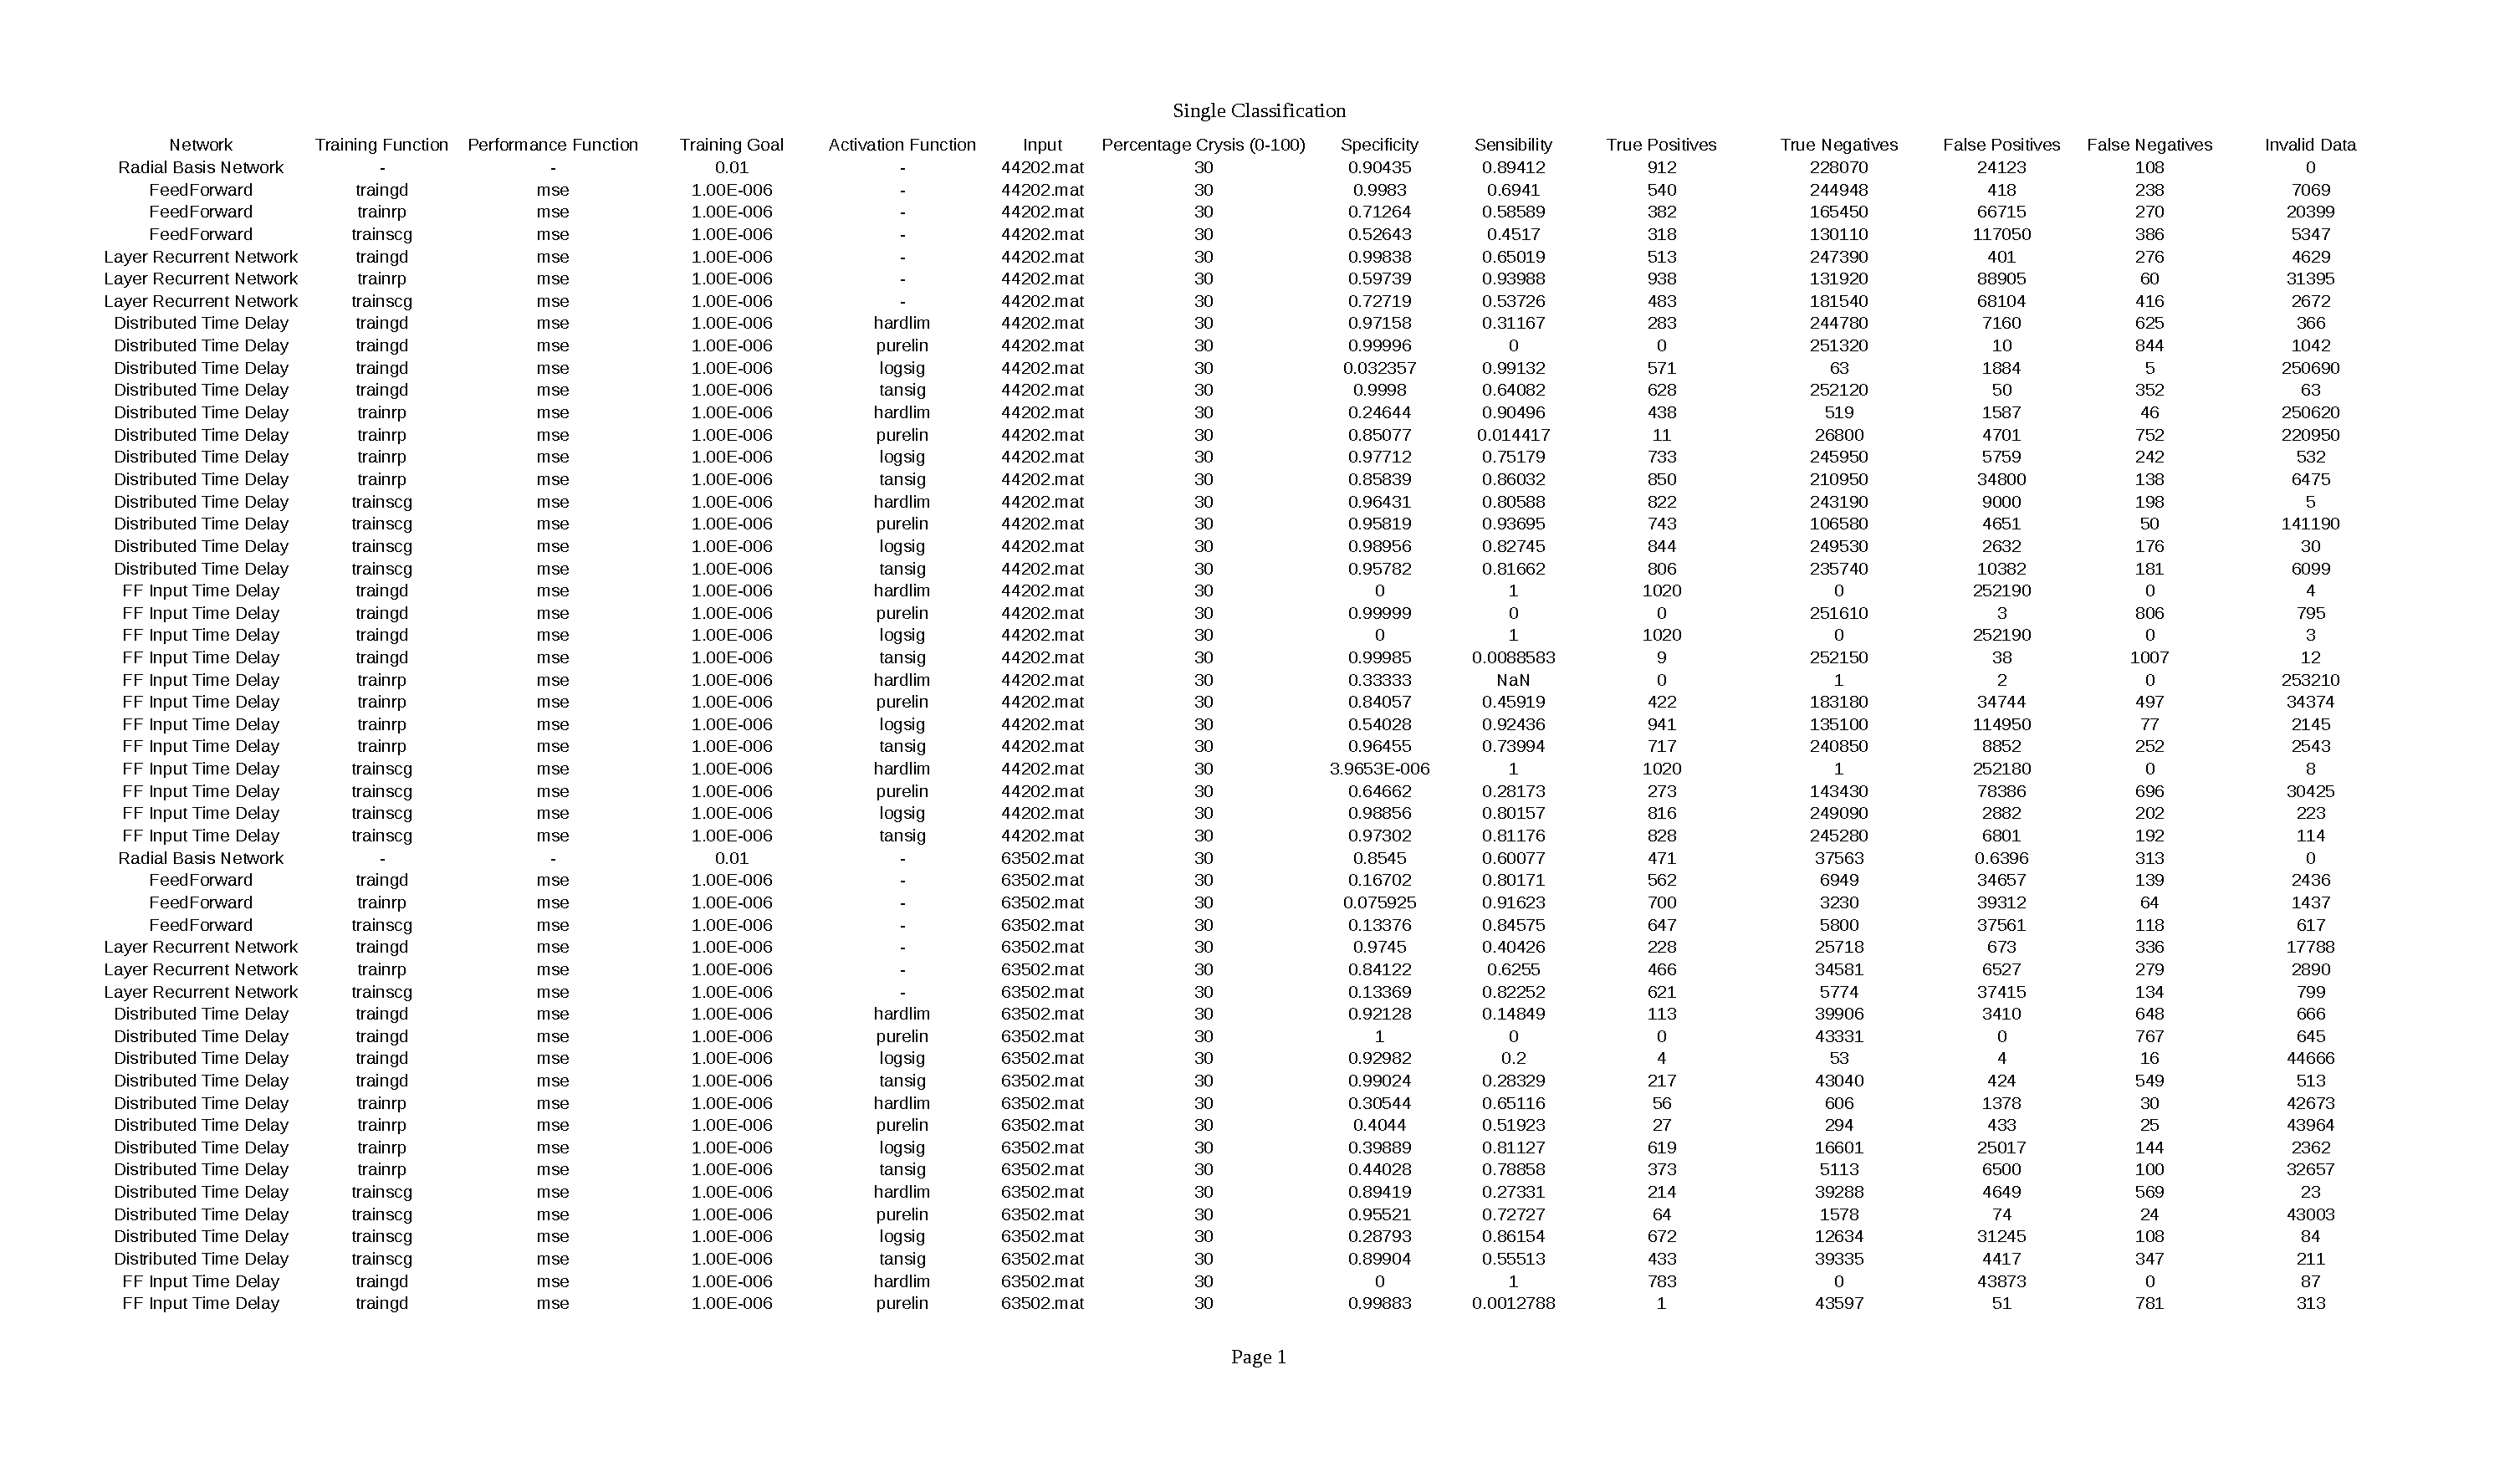
\includepdf[pages={1-10}]{Images/Results.pdf}

Nas páginas seguintes apresentamos os testes posteriores realizados às redes que apresentaram melhores resultados nos testes iniciais, conforme o descrito na \emph{Secção}~\ref{sec:train_tests} deste documento.

\includepdf[pages={11-14}]{Images/Results.pdf}

\end{document}